\documentclass[master.tex]{subfiles}
\begin{document}

\chapter{Example --- Simple Arithmetic}
\label{chap:example_simple_arithmetic}

As in \hyperref[chap:background]{background chapter}, simple arithmetic is
used as example to explain basic concept of formal systems and its derivations.
In order to make the transition goes smoother, this chapter aims to encode
simple arithmetic into phometa. Please note that this is just a faction of
actual arithmetic modified to make it easy to understand, so it is not as
powerful as the actual one.

\section{First time with phometa}

You can download complied version of phometa at

{\centering\url{https://github.com/gunpinyo/phometa/raw/master/build/phometa.tar.gz}}

Once you unzip this file, you can start phometa server by execute

\texttt{./phometa-server.py 8080}

where \texttt{8080} is port number, you can change this to another port number
if you like. Please note that python is required for this server.

Then open your favourite web-browser\footnote{but Google Chrome is recommended}
and enter

\texttt{http://localhost:8080/phometa.html}

The program will look like this

\begin{figure}[H]
    \centering
    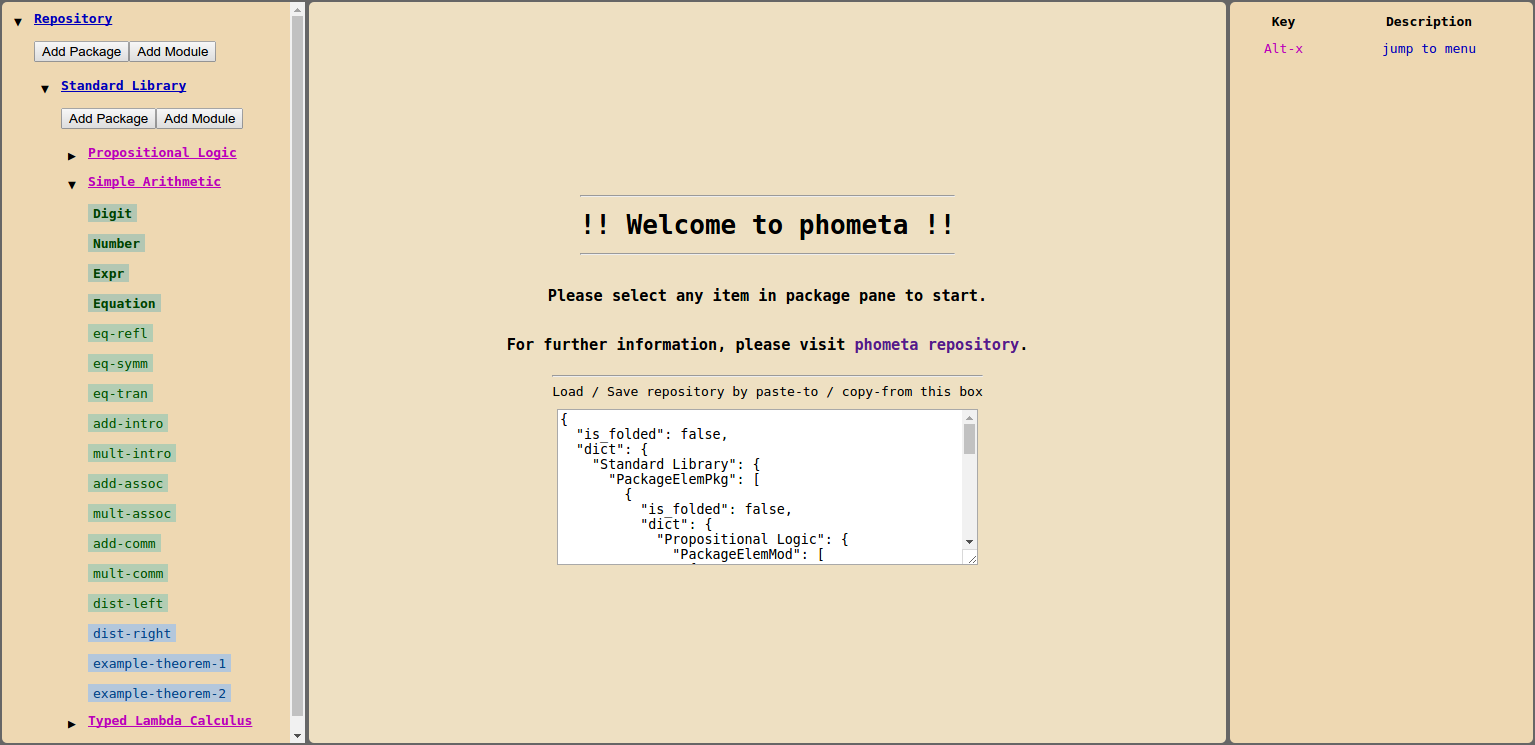
\includegraphics[width=0.85\textwidth]{arith-phometa-home-window}
    \caption{Screenshot of Phometa when you open it from web-browser.}
\label{fig:arith-phometa-home-window}
\end{figure}

Phometa has a repository which consists of packages and modules that store
formal systems and its proofs. The left pane of figure
\ref{fig:arith-phometa-home-window} shows global structure of a repository. The
current repository has one package named ``Standard Library'' which consists of
three modules named ``Propositional Logic'', ``Simple Arithmetic'', and ``Typed
Lambda Calculus''.

Module in phometa are analogous to text file. It consists of nodes that could
depend on one another. There are four types of node which are \emph{Comment},
\emph{Grammar} (Backus-Naur Form), \emph{Rule} (Derivation Rule), and
\emph{Theorem} (Derivation Tree). If you click at a module on the repository
pane e.g. ``Simple Arithmetic'', you will see the whole content of the module
appear on the centre pane. Alternatively, you can click on each node on the
repository pane directly to focus on particular node.

\begin{figure}[H]
    \centering
    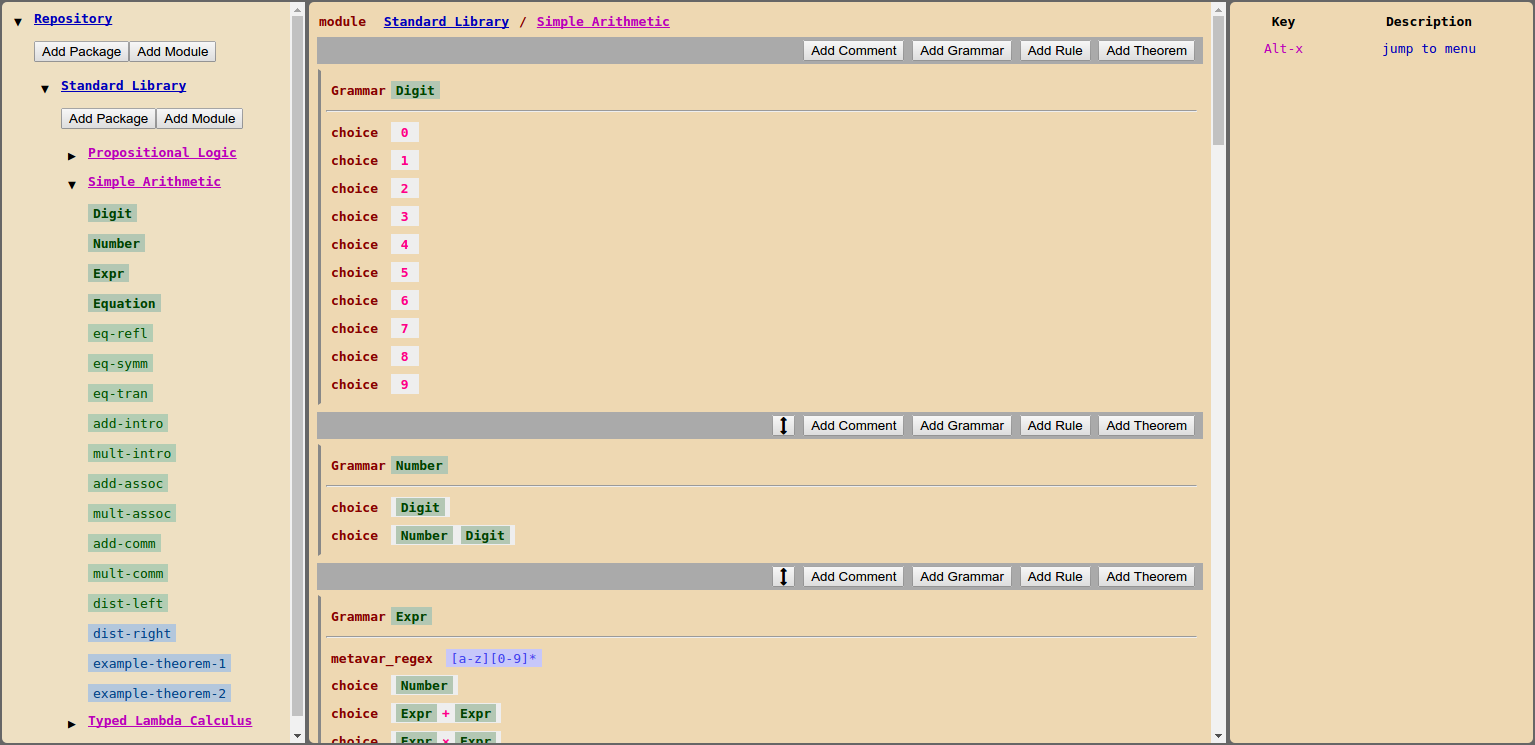
\includegraphics[width=0.85\textwidth]{arith-phometa-arith-window}
    \caption{Screenshot of Phometa when you click ``Simple Arithmetic'' module.}
\label{fig:arith-phometa-arith-window}
\end{figure}

In order to improve productivity, phometa has several key-bindings specific to
curtain state of program. Fortunately, user don't need to remember any of this
since the right pane (i.e. keymap pane) shows every possible key-binding with
its description on current state. This also allow new-comer to explore new
features during using it

\section{Grammars}

The Backus-Naur Form of simple arithmetic in figure \ref{fig:background-bnf}
could be transformed in to this four following grammars
\begin{figure}[H]
    \centering
\begin{minipage}{0.48\textwidth}
\begin{flushleft}
    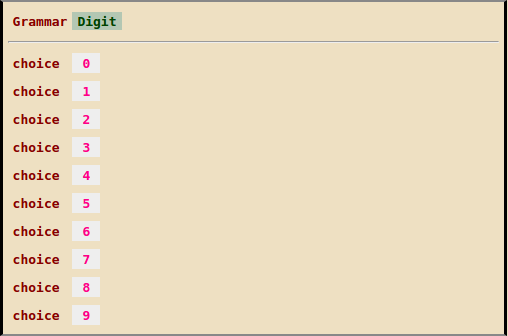
\includegraphics[width=\textwidth]{arith-grammar-digit}
\end{flushleft}
\end{minipage}
~
\begin{minipage}{0.48\textwidth}
\begin{flushright}
    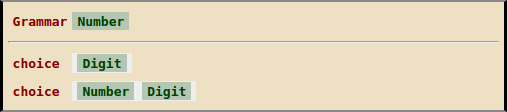
\includegraphics[width=\textwidth]{arith-grammar-number}
    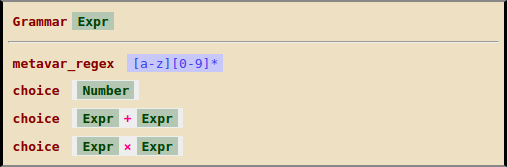
\includegraphics[width=\textwidth]{arith-grammar-expr}
    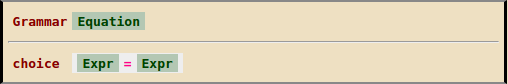
\includegraphics[width=\textwidth]{arith-grammar-equation}
\end{flushright}
\end{minipage}
    \caption{Grammars of Simple Arithmetic}
\label{fig:arith-grammars}
\end{figure}

We take advantage of visualisation by replacing brackets with underlines, this
should improve readability because reader can see a whole term in a compact
way but still able check how they are bounded when needed, for example,
\begin{itemize}
\item \texttt{<Number>} $250$ is transformed to
  \pgmr{Number} \bat{\bat{\bat{\bat{$2$}} \bat{$5$}} \bat{$0$}}
\item \texttt{<Expr>} $(0 + (12 \times 6))$ is transformed to
  \pgmr{Expr} \bat{\bat{\bat{\bat{$0$}}} $+$ \bat{\bat{\bat{\bat{\bat{$1$}} \bat{$2$}}} $\times$ \bat{\bat{\bat{$6$}}}}}
\item \texttt{<Equation>} $(5 + 7) = 12$ is transformed to
  \pgmr{Equation} \bat{\bat{\bat{\bat{\bat{$5$}}} $+$ \bat{\bat{\bat{$7$}}}} $=$ \bat{\bat{\bat{\bat{$1$}} \bat{$2$}}}}
\end{itemize}
These underline patterns coincide with diagram in figures
\ref{fig:background-number}, \ref{fig:background-expr}, and
\ref{fig:background-equation} respectively.

\kMetaVarRegex\ is used to control the name meta variables of each grammar. If
this property is omitted, the corresponding grammar cannot instantiate meta
variables. For example, \pgmr{Expr} can instantiate meta variables with the name
comply to regular expression \pregex{\texttt{[a-z][0-9]*}} (e.g. \pvar{a}, \pvar{b},
$\ldots$, \pvar{z}, \pvar{a1}, \pvar{a2}, $\ldots$), whereas \pgmr{Digit},
\pgmr{Number}, and \pgmr{Equation} couldn't instantiate any meta variables,
however, it could have meta variables as sub-term e.g. \pgmr{Equation}
\bat{\bat{\pvar{x} $+$ \pvar{x}} $=$ \bat{\bat{\bat{\bat{$2$}}} $\times$ \pvar{x}}}.

\section{Rules}

The derivation rules of simple arithmetic in figure \ref{fig:background-derivation-rules}
could be transformed as the following

\pthm{dist-right} is not defined here but it will be defined as \emph{lemma}
in the next section.

\section{Theorems}

\end{document}